%===============================================================================
% LaTeX sjabloon voor de bachelorproef toegepaste informatica aan HOGENT
% Meer info op https://github.com/HoGentTIN/latex-hogent-report
%===============================================================================

\documentclass[dutch,dit,thesis]{hogentreport}

\usepackage{lipsum} % For blind text, can be removed after adding actual content

%% Pictures to include in the text can be put in the graphics/ folder
\graphicspath{{graphics/}}

%% For source code highlighting, requires pygments to be installed
%% Compile with the -shell-escape flag!
\usepackage[section]{minted}
%% If you compile with the make_thesis.{bat,sh} script, use the following
%% import instead:
%% \usepackage[section,outputdir=../output]{minted}
\usemintedstyle{solarized-light}
\definecolor{bg}{RGB}{253,246,227} %% Set the background color of the codeframe

%% Change this line to edit the line numbering style:
\renewcommand{\theFancyVerbLine}{\ttfamily\scriptsize\arabic{FancyVerbLine}}

%% Macro definition to load external java source files with \javacode{filename}:
\newmintedfile[javacode]{java}{
    bgcolor=bg,
    fontfamily=tt,
    linenos=true,
    numberblanklines=true,
    numbersep=5pt,
    gobble=0,
    framesep=2mm,
    funcnamehighlighting=true,
    tabsize=4,
    obeytabs=false,
    breaklines=true,
    mathescape=false
    samepage=false,
    showspaces=false,
    showtabs =false,
    texcl=false,
}

% Other packages not already included can be imported here

%%---------- Document metadata -------------------------------------------------
% TODO: Replace this with your own information
\author{Max Milan}
\supervisor{Dhr. G. Bosteels}
\cosupervisor{Dhr. A. Pannemans}
\title%[Optionele ondertitel]%
    {Geautomatiseerde documentatie generatie met behulp van Large Language Modellen: Het genereren van duidelijke overzichten en informatieve beschrijvingen voor Python projecten}
\academicyear{\advance\year by -1 \the\year--\advance\year by 1 \the\year}
\examperiod{1}
\degreesought{\IfLanguageName{dutch}{Professionele bachelor in de toegepaste informatica}{Bachelor of applied computer science}}
\partialthesis{false} %% To display 'in partial fulfilment'
%\institution{Internshipcompany BVBA.}

%% Add global exceptions to the hyphenation here
\hyphenation{back-slash}

%% The bibliography (style and settings are  found in hogentthesis.cls)
\addbibresource{bachproef.bib}            %% Bibliography file
\addbibresource{../voorstel/voorstel.bib} %% Bibliography research proposal
\defbibheading{bibempty}{}

%% Prevent empty pages for right-handed chapter starts in twoside mode
\renewcommand{\cleardoublepage}{\clearpage}

\renewcommand{\arraystretch}{1.2}

%% Content starts here.
\begin{document}

%---------- Front matter -------------------------------------------------------

\frontmatter

\hypersetup{pageanchor=false} %% Disable page numbering references
%% Render a Dutch outer title page if the main language is English
\IfLanguageName{english}{%
    %% If necessary, information can be changed here
    \degreesought{Professionele Bachelor toegepaste informatica}%
    \begin{otherlanguage}{dutch}%
       \maketitle%
    \end{otherlanguage}%
}{}

%% Generates title page content
\maketitle
\hypersetup{pageanchor=true}

%%=============================================================================
%% Voorwoord
%%=============================================================================

\chapter*{\IfLanguageName{dutch}{Woord vooraf}{Preface}}%
\label{ch:voorwoord}

%% TODO:
%% Het voorwoord is het enige deel van de bachelorproef waar je vanuit je
%% eigen standpunt (``ik-vorm'') mag schrijven. Je kan hier bv. motiveren
%% waarom jij het onderwerp wil bespreken.
%% Vergeet ook niet te bedanken wie je geholpen/gesteund/... heeft

Toen ik aan de richting Toegepaste Informatica begon, wist ik meteen welke specialisatie ik wilde volgen: AI en Data Engineering sprak mij direct aan. 
Deze richting biedt mij de mogelijkheid om steeds nieuwe uitdagingen te vinden in alles wat ik doe.

Het hebben van een uitdaging geeft mij de motivatie om steeds het beste van mezelf te geven. 
Zo was het ook een uitdaging om deze bachelorproef tot een goed einde te brengen. 
Een van de grootste uitdagingen was het werken met LLM's, aangezien dit de eerste keer was dat ik deze zelf implementeerde.

Daarom wil ik graag mijn co-promotor, Arne Pannemans, bedanken voor zijn onophoudelijke steun en waardevolle bijdragen. 
Uw voortdurende aanwezigheid bij het geven van feedback en uw kritische blik waren van onschatbare waarde voor het tot stand brengen van deze bachelorproef. 
Uw continue steun en toewijding hebben mij geïnspireerd en gemotiveerd om het beste uit mezelf te halen. 
Dankzij uw begeleiding heb ik mijn onderzoek naar een hoger niveau kunnen tillen.

Ook wil ik mijn promotoren meneer Gert-Jan Bosteels en mevrouw Lena De Mol bedanken voor hun kritische en waardevolle feedback. 
Deze feedback heeft ervoor gezorgd dat ik de juiste richting uitging en dat ik mijn ideeën helder kon verwoorden.

Tot slot zou ik graag mijn ouders en vrienden willen bedanken. Hun steun, voortdurende aanmoediging en begrip hebben mij door alle moeilijke momenten geholpen. 
Dankzij hen heb ik deze bachelorproef tot een goed einde kunnen brengen.

%%=============================================================================
%% Samenvatting
%%=============================================================================

% TODO: De "abstract" of samenvatting is een kernachtige (~ 1 blz. voor een
% thesis) synthese van het document.
%
% Een goede abstract biedt een kernachtig antwoord op volgende vragen:
%
% 1. Waarover gaat de bachelorproef?
% 2. Waarom heb je er over geschreven?
% 3. Hoe heb je het onderzoek uitgevoerd?
% 4. Wat waren de resultaten? Wat blijkt uit je onderzoek?
% 5. Wat betekenen je resultaten? Wat is de relevantie voor het werkveld?
%
% Daarom bestaat een abstract uit volgende componenten:
%
% - inleiding + kaderen thema
% - probleemstelling
% - (centrale) onderzoeksvraag
% - onderzoeksdoelstelling
% - methodologie
% - resultaten (beperk tot de belangrijkste, relevant voor de onderzoeksvraag)
% - conclusies, aanbevelingen, beperkingen
%
% LET OP! Een samenvatting is GEEN voorwoord!

%%---------- Samenvatting -----------------------------------------------------
% De samenvatting in de hoofdtaal van het document

\chapter*{\IfLanguageName{dutch}{Samenvatting}{Abstract}}

Deze bachelorproef richt zich op het documenteren van ongedocumenteerde\\ Python-projecten met behulp van een Large Language Model (LLM).
Het genereren van duidelijk en overzichtelijke documentatie van een project helpt bij het begrijpen van de code en is de eerste stap in het delen van kennis.
Bestaande tools hebben echter gedocumenteerde code nodig om documentatie te genereren. 
Het automatiseren van het documentatieproces zorgt ervoor dat dit geen manuele taak meer is.  

De centrale onderzoeksvraag is: "Hoe kan geautomatiseerde documentatiegeneratie met behulp van Large Language Modellen (LLM) effectief worden toegepast op ongedocumenteerde Python-projecten om er duidelijke en overzichtelijke documentatie van te maken?" 
Deze vraag is verder opgesplitst in enkele deelvragen, wat is documentatie en wat is er nodig om een bestand en een project te documenteren?
Met als doel een Proof of Concept (PoC) van een geautomatiseerde tool die de code van een Python-project analyseert en er documentatie van genereert.

Het onderzoek omvat enkele fases. Eerst wordt er gekeken hoe een enkel bestand gedocumenteerd kan worden. 
Vervolgens wordt er gekeken hoe verschillende bestanden in een project samen gedocumenteerd kunnen worden om zo een overzicht van het project te geven.
De laatste fase beslaagt het evalueren van de tool door de documentatie van de tool te vergelijken met de handgeschreven documentatie van een project.

De resultaten van de evaluatie tonen aan dat de documentatie van de tool en de handgeschreven documentatie gelijkaardig zijn en door de visuele weergave van de relaties tussen de bestanden is de documentatie overzichtelijk en duidelijk.
Er kunnen echter wel enkele fouten in de documentatie sluipen.

Deze studie biedt een oplossing voor het documenteren van ongedocumenteerde Python-projecten en kan gebruikt worden om de kennis van een project te delen met anderen.


%---------- Inhoud, lijst figuren, ... -----------------------------------------

\tableofcontents

% In a list of figures, the complete caption will be included. To prevent this,
% ALWAYS add a short description in the caption!
%
%  \caption[short description]{elaborate description}
%
% If you do, only the short description will be used in the list of figures

\listoffigures

% If you included tables and/or source code listings, uncomment the appropriate
% lines.
%\listoftables
%\listoflistings

% Als je een lijst van afkortingen of termen wil toevoegen, dan hoort die
% hier thuis. Gebruik bijvoorbeeld de ``glossaries'' package.
% https://www.overleaf.com/learn/latex/Glossaries

%---------- Kern ---------------------------------------------------------------

\mainmatter{}

% De eerste hoofdstukken van een bachelorproef zijn meestal een inleiding op
% het onderwerp, literatuurstudie en verantwoording methodologie.
% Aarzel niet om een meer beschrijvende titel aan deze hoofdstukken te geven of
% om bijvoorbeeld de inleiding en/of stand van zaken over meerdere hoofdstukken
% te verspreiden!

%%=============================================================================
%% Inleiding
%%=============================================================================

\chapter{\IfLanguageName{dutch}{Inleiding}{Introduction}}%
\label{ch:inleiding}

De inleiding moet de lezer net genoeg informatie verschaffen om het onderwerp te begrijpen en in te zien waarom de onderzoeksvraag 
de moeite waard is om te onderzoeken. In de inleiding ga je literatuurverwijzingen beperken, zodat de tekst vlot leesbaar blijft. 
Je kan de inleiding verder onderverdelen in secties als dit de tekst verduidelijkt. 
Zaken die aan bod kunnen komen in de inleiding~\autocite{Pollefliet2011}:

\begin{itemize}
  \item context, achtergrond
  \item afbakenen van het onderwerp
  \item verantwoording van het onderwerp, methodologie
  \item probleemstelling
  \item onderzoeksdoelstelling
  \item onderzoeksvraag
  \item \ldots
\end{itemize}

\section{\IfLanguageName{dutch}{Probleemstelling}{Problem Statement}}%
\label{sec:probleemstelling}

Projecten worden vaak niet goed gedocumenteerd, dit kan leiden tot problemen in de toekomst. Wanneer een andere persoon de code van een ongedocumenteerd project wilt gebruiken moet de code volledig gelezen worden voordat er begrepen wordt wat de code doet. 
Dit is een tijdrovend proces en kan voorkomen worden door goede documentatie.
Wanneer de code jaren later aangepast moet worden is het ook handig om goede documentatie te hebben, zodat de persoon weet waar er aanpassingen moeten gebeuren.
De skills en know-how van een project kunnen verloren gaan wanneer er geen documentatie is.
Deze dienen juist gedeeld te worden met anderen zodat er geen dubbel werk gedaan moet worden.
Het is dus belangrijk dat er aan documentatie gedaan wordt en dat deze up-to-date blijft.

Het documenteren van een project is iets wat veel tijd kost en wat meestal geen aandacht krijgt.
Een tool die dit proces kan versnellen / automatiseren zou een grote meerwaarde zijn.
De tool bestaat uit een geautomatiseerde documentatie LLM die de project code analyseert en samenvat in een document. 
Dit geeft de lezers de mogelijkheid om zich in te lezen in het project en erna zelf aanpassingen te maken of stukken code te gebruiken voor een ander project.

\section{\IfLanguageName{dutch}{Onderzoeksvraag}{Research question}}%
\label{sec:onderzoeksvraag}

Hoe kan geautomatiseerde documentatiegeneratie met behulp van Large Language Modellen (LLM) effectief worden toegepast om duidelijke en informatieve overzichten te produceren voor Python projecten?

\section{\IfLanguageName{dutch}{Onderzoeksdoelstelling}{Research objective}}%
\label{sec:onderzoeksdoelstelling}

Het eindresultaat van deze bachelorproef is een Proof of Concept (PoC) van een geautomatiseerde tool die de project code analyseert en er documentatie van genereert.
De gegenereerde documentatie laat het toe het project te begrijpen zonder er te veel tijd aan te besteden.

\section{\IfLanguageName{dutch}{Opzet van deze bachelorproef}{Structure of this bachelor thesis}}%
\label{sec:opzet-bachelorproef}

% Het is gebruikelijk aan het einde van de inleiding een overzicht te
% geven van de opbouw van de rest van de tekst. Deze sectie bevat al een aanzet
% die je kan aanvullen/aanpassen in functie van je eigen tekst.

De rest van deze bachelorproef is als volgt opgebouwd:

In Hoofdstuk~\ref{ch:stand-van-zaken} wordt een overzicht gegeven van de stand van zaken binnen het onderzoeksdomein, op basis van een literatuurstudie.

In Hoofdstuk~\ref{ch:methodologie} wordt de methodologie toegelicht en worden de gebruikte onderzoekstechnieken besproken om een antwoord te kunnen formuleren op de onderzoeksvragen.

% TODO: Vul hier aan voor je eigen hoofstukken, één of twee zinnen per hoofdstuk

In Hoofdstuk~\ref{ch:conclusie}, tenslotte, wordt de conclusie gegeven en een antwoord geformuleerd op de onderzoeksvragen. Daarbij wordt ook een aanzet gegeven voor toekomstig onderzoek binnen dit domein.
\chapter{\IfLanguageName{dutch}{Stand van zaken}{State of the art}}%
\label{ch:stand-van-zaken}

% Tip: Begin elk hoofdstuk met een paragraaf inleiding die beschrijft hoe
% dit hoofdstuk past binnen het geheel van de bachelorproef. Geef in het
% bijzonder aan wat de link is met het vorige en volgende hoofdstuk.

% Pas na deze inleidende paragraaf komt de eerste sectiehoofding.

In dit hoofdstuk wordt de literatuurstudie besproken. 
Door deze literatuurstudie is het mogelijk om een beter inzicht te krijgen in de technologie en mogelijkheden voor de documentatie van Python-projecten alsook hoe het toegepast kan worden met behulp van Large Language Modellen. 
Er zal nadruk worden gelegd op bestaande literatuur en onderzoeken die verbonden zijn met documentatie van Python-projecten. 
In dit onderdeel zullen verschillende hoofdstukken worden aangekaart. 
Als eerste zal er duidelijk gemaakt worden wat er juist verstaan wordt onder documentatie. 
Vervolgens wordt er gekeken naar bestaande documentatie tools.
In het derde deel van deze literatuurstudie wordt er gekeken wat Large Language Modellen zijn, hoe deze werken en wat enkele bestaande modellen zijn.

\section{Wat is documentatie?}
\label{sec:wat-is-documentatie}

Alvorens dieper op het onderwerp in te gaan, is het belangrijk dat er een duidelijk beeld gevormd wordt wat documentatie is. 
Waarom is documentatie belangrijk voor een project en wat wordt er begrepen onder documentatie? 

Documentatie is het proces van het vastleggen van de werking van een project.
Volgens \textcite{CodeQuality2024} kan dit op verschillende manieren gebeuren. 
Er kan gekozen worden om de documentatie te schrijven in de vorm van een commentaar in de code, een docstring, een API voor klassen of functies of in de vorm van een README.md bestand \autocite{CodeQuality2024}.
Het doel van documentatie is om de werking van het project te beschrijven zodat andere programmeurs het project kunnen begrijpen en gebruiken.
Zo gaat er geen tijd verloren aan het lezen van de code en het begrijpen ervan.

Documentatie kan gemaakt worden voor verschillende doelgroepen. Het kan voor interne of externe doeleinden zijn.
Interne documentatie is voor documentatie binnen hetzelfde bedrijf.
Dit gaat dan om het capteren van de proces kennis die vergaard is binnen een project. Dit is informatie zoals een roadmap of product requirements. 
Deze documentatie gaat over het vastleggen van gedetaïlleerde uitleg over hoe iets werkt en hoe het onderhouden kan worden \autocite{swimm.io2024}.

Externe documentatie is voor documentatie die gedeeld wordt met andere bedrijven of klanten. 
Dit gaat dan over de basiswerking van de code van een project zodat andere programmeurs het kunnen gebruiken.
Gebruiksaanwijzingen of handleidingen zijn ook een vorm van externe documentatie \autocite{swimm.io2024}.

Voor deze bachelorproef wordt er gekeken naar het documenteren van een Python-project in de vorm van commentaar in de code en het genereren van een samenvattend document van het gehele project.
Omdat Python een populaire programmeertaal is volgens \textcite{TIOBE2024} en er veel projecten in deze taal geschreven worden, is het interessant om te kijken hoe deze projecten gedocumenteerd kunnen worden.
Ook kan er in de code bij functies aan type hinting gedaan worden. Dit indiceert wat de datatypes van de input en output van een functie zijn \autocite{Bailey2024}.
Uit deze documentatie kan de werking van het project duidelijk worden en kunnen de relaties tussen de verschillende bestanden en functies weergegeven worden.

In het verdere verloop van deze bachelorproef wordt er gekeken hoe de documentatie van een Python-project gegenereerd kan worden.

\subsection{Bestand documentatie}
\label{sec:bestand-documentatie}
Eerst dienen de bestanden van het project gedocumenteerd te worden.
Dit gebeurt door de code van het bestand te analyseren en de docstrings van de verschillende functies en klassen te genereren.

Docstrings of documentatie strings worden aan het begin van een functie of klasse geplaatst.
Deze strings worden gebruikt om de functie of klasse te documenteren \autocite{GeeksforGeeks2023}.
Volgens \textcite{GeeksforGeeks2023} zijn docstrings vitaal in het overdragen van het doel en de werking van een functie of klasse.

Deze docstrings kunnen dan gebruikt worden om een samenvatting van het bestand te genereren.

\subsection{Project documentatie}
\label{sec:project-documentatie-literatuur}
De documentatie van het project wordt gemaakt door de samenvattingen van de verschillende bestanden te combineren.
Deze samenvattingen worden gegenereerd op basis van de samenvatting van de bestanden die tot het project behoren.
In deze samenvatting behoort de werking van het project, de verschillende bestanden met functies en klassen en de relaties tussen deze bestanden.


\section{Bestaande documentatie tools}
\label{sec:huidige-tools}
Voor er gekeken wordt hoe LLM's mogelijk gebruikt kunnen worden voor het genereren van documentatie is het belangrijk dat er een helder beeld is van de huidige tools die gebruikt worden voor het genereren van documentatie.
De documentatie kan in verschillende vormen gegeneerd worden. Dit kan gaan van een website tot een samenvattend document.
Ook kunnen er in de code zelf commentaren geplaatst worden die de werking van de code uitleggen.
Hiervoor bestaan er reeds verschillende tools en dit voor verschillende programmeertalen opgelijst in tabel \ref{table:vgl-tools}.
In dit onderdeel is er enkel gekeken naar tools die nog onderhouden worden door de makers. 

\subsection{Doxygen}
Doxygen \autocite{Doxygen2023} is een tool die het toelaat om automatisch code documentatie te genereren. Het is een gratis tool die bruikbaar is voor verschillende programmeertalen zoals: C++, C, Python, PHP en Java.
Het genereert documentatie in de vorm van HTML, LaTeX, RT. 
Deze tool is in staat om een diagram te genereren met de relaties tussen de verschillende delen van de code bijvoorbeeld de relaties tussen de verschillende klassen en functies.
Een voorbeeld van een diagram kan gezien worden in figuur \ref{fig:Doxygen-diagram}.
Zo wordt er een duidelijk beeld verkregen van de structuur van het project.

\begin{figure}[h]
  \centering
  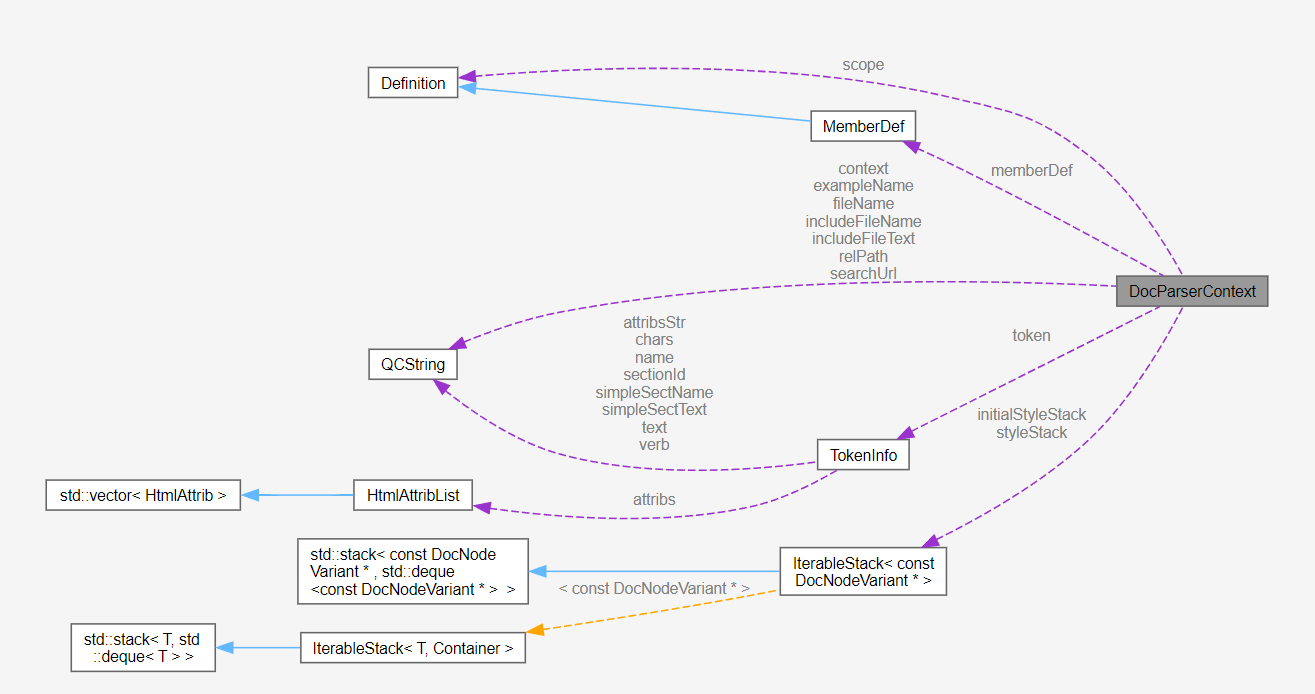
\includegraphics[width=1\textwidth]{doxygen_diagram.png}
  \caption{Voorbeeld diagram van Doxygen \autocite{Doxygen2023}}
  \label{fig:Doxygen-diagram}
\end{figure}

\subsection{CodeCat}
\textcite{CodeCat2024} is een online tool die de code analyseert en de docstrings genereert. Er kan niet gekeken worden naar de werking van CodeCat aangezien het niet open sourced is.
Deze tool genereert automatisch de docstrings voor JavaScript code.

\subsection{GPT4Docstrings}
De tool van \textcite{Trofficus2023} genereert docstrings voor Python code. Het maakt gebruik van GPT-4 \autocite{OpenAI2023} om de docstrings te genereren.
Deze tool leunt sterk aan bij de doelstelling van deze bachelorproef, namelijk het genereren van documentatie met behulp van LLM's.
Het nader bekijken van deze tool kan een meerwaarde zijn voor deze bachelorproef.

\begin{figure}
  \centering
  \begin{subfigure}[b]{0.5\textwidth}
      \centering
      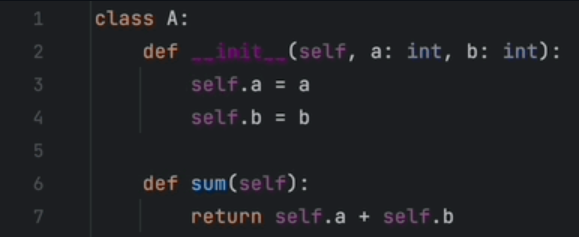
\includegraphics[width=1\textwidth]{before_troficus.png}
      \caption{Voorbeeld code zonder docstrings van \textcite{Trofficus2023}}
      \label{fig:before-Trofficus}
  \end{subfigure}
  \hfill
  \begin{subfigure}[b]{0.5\textwidth}
      \centering
      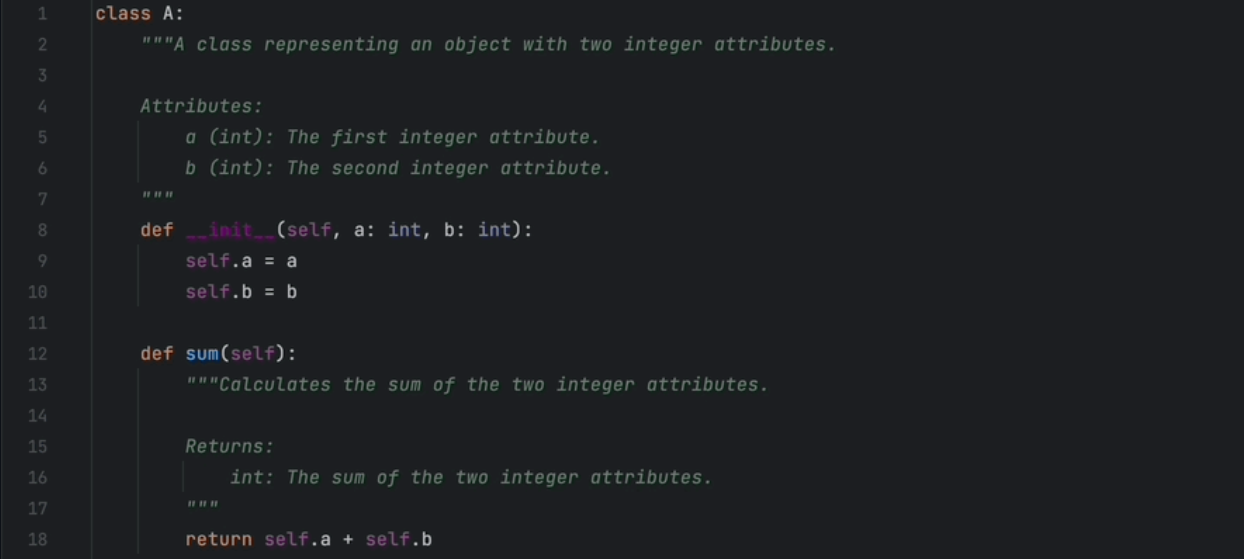
\includegraphics[width=1\textwidth]{after_troficus.png}
      \caption{Voorbeeld code met docstrings van \textcite{Trofficus2023}}
      \label{fig:after-Trofficus}
  \end{subfigure}
     \caption[Uitkomst GPT4Docstrings]{Voorbeeld uitkomst van de tool van \textcite{Trofficus2023}}
     \label{fig:Before-After-Trofficus}
\end{figure}

Zo gebruikt GPT4Docstrings van \textcite{Trofficus2023} de Abstract Syntax Tree (AST) van de code om de structuur van de code te begrijpen.
Uit de AST kunnen de juiste stukken code gehaald worden om de docstrings te genereren.
Dit kan goed van pas komen voor het genereren van documentatie van Python-projecten.
Een voorbeeld van deze tool kan gezien worden in figuur \ref{fig:Before-After-Trofficus}. 

\subsection{Sphinx}
Sphinx van \textcite{Sphinx2023} is één van de meest gebruikte tools voor het genereren van documentatie voor Python-projecten.
Het genereert documentatie aan de hand van docstrings. Het toont de hiërarchie van het project om een duidelijk overzicht te geven.
Deze tool is vrij flexibel want het kan uitgebreid worden met verschillende extensies, zodat het alle mogelijke wensen kan vervullen.
Volgens \textcite{Sphinx2023} kan de extensie autodoc semi-automatisch de docstrings van een module extraheren en in de documentatie plaatsen. 
Dit is handig wanneer de automatische documentatie generatie van een geheel project gewenst is. Zo kan het project samengevat worden aan de hand van de docstrings van de verschillende python files. 
Alvorens een Python-project gedocumenteerd kan worden met Sphinx \autocite{Sphinx2023} dienen alle bestanden aangevuld te worden met docstrings.
Dit gebeurt echter niet bij het runnen van het programma.

\subsection{Pdoc}
Pdoc \autocite{GallantHils2023} genereert documentatie in de vorm van een website die een API van de documentatie bevat. 
Hier kan er eenvoudig op de website gezocht worden naar een functie of klasse met de bijhorende documentatie.

\begin{table}[h!]
\centering
\resizebox{\textwidth}{!}{
\begin{tabular}{|c|c|c|}
\hline
Tool & programmeertaal & type \\ [0.5ex]
\hline
Doxygen & C++, C, Python, PHP, Java & HTML, PDF, markdown\\
\hline
CodeCat & JavaScript & docstring \\
\hline
Sphinx & Python & HTML, LATEX, man pages \\
\hline
Pdoc & Python & API \\
\hline
GPT4Docstrings & Python & docstring \\
\hline
\end{tabular}}
\caption{Vergelijking documentatie tools}
\label{table:vgl-tools}
\end{table}

\subsection{Samenvatting tools}
\label{sec:samenvatting-tools}
Door de verschillende tools op te lijsten en te vergelijken met elkaar wordt er een duidelijk beeld gevormd wat de tools kunnen genereren.
Zo kan er een keuze gemaakt worden welke tool het beste past bij dit onderzoek.
In tabel \ref{table:ra-tools} wordt er een overzicht gegeven wat de tools kunnen genereren.
De tools Doxygen, Sphinx en Pdoc kunnen enkel een document genereren in de vorm van een website of een bestand op basis van reeds bestaande docstrings en commentaren in de code.
De tool GPT4Docstrings genereert docstrings voor Python code met behulp van een LLM.

\begin{table}[h!]
  \centering
  \resizebox{\textwidth}{!}{
  \begin{tabular}{|c|c|c|c|c|}
  \hline
  Tool & docstrings & samenvatting bestand & samenvatting project & visualisatie \\ [0.5ex]
  \hline
  GPT4Docstrings & ja & nee & nee & nee \\
  \hline
  Doxygen & nee & nee & nee & ja \\
  \hline
  Sphinx & nee & nee & nee & nee \\
  \hline
  Pdoc & nee & nee & nee & nee \\
  \hline
  \end{tabular}}
  \caption{Overzicht van wat de tools kunnen genereren}
  \label{table:ra-tools}
  \end{table}

\section{Wat zijn Large Language Modellen (LLM)?}
\label{sec:wat-zijn-llms}

Uit de vorige sectie is gebleken dat er slechts één tool geschikt is voor het genereren van documentatie voor projecten zonder gedocumenteerde code. 
De tool GPT4Docstrings van \textcite{Trofficus2023} maakt gebruik van een Large Language Model (LLM) om de docstrings te genereren.
Het is dus belangrijk dat er een duidelijk beeld is van wat LLM's juist zijn en hoe deze werken.
Wat kunnen deze modellen, wat zijn de mogelijke beperkingen en wat is de huidige stand van zaken. 
In dit hoofdstuk wordt er een antwoord gegeven op de vragen: 
\begin{itemize}
  \item Bestaan er LLM's speciaal getraind op Python code? 
  \item Kunnen LLM's gebruikt worden om documentatie te genereren?
\end{itemize}

Dit draagt bij tot het verkrijgen van een grondige basiskennis van LLM's. 
Het veld waarin AI zich bevindt, wordt vaak voorgesteld volgens figuur \ref{fig:LLM-position}. Het bestaat uit verschillende cirkels met elk een eigen laag volgens \textcite{Stoeffelbauer2023}.
Deze lagen zijn: Artificiële Intelligentie, Machine Learning, Deep Learning en Large Language Modellen.
Omdat LLM's een subveld zijn van Deep Learning is het belangrijk dat er een duidelijk beeld is van wat Deep Learning juist is.
Uit de figuur \ref{fig:LLM-position} blijkt dat AI verschillende categorieën omvat.
Volgens \textcite{Stoeffelbauer2023} is AI een brede term wat vaak verwijst naar slimme machines. 
Machine Learning (ML) is een subveld van AI, waarin patronen worden herkend tussen een input en een output.
ML kan gebruikt worden voor verschillende taken zoals classificatie, regressie, clustering en dergelijke.
Volgens \textcite{Stoeffelbauer2023} is Deep Learning (DL) een subveld van ML, waarin complexe algoritmen en Deep Neural Networks gebruikt worden om complexere taken uit te voeren.
Deep Learning is een krachtige tool die gebruikt wordt voor verschillende taken zoals: beeldherkenning, spraakherkenning, ...

\begin{figure}[h]
  \centering
  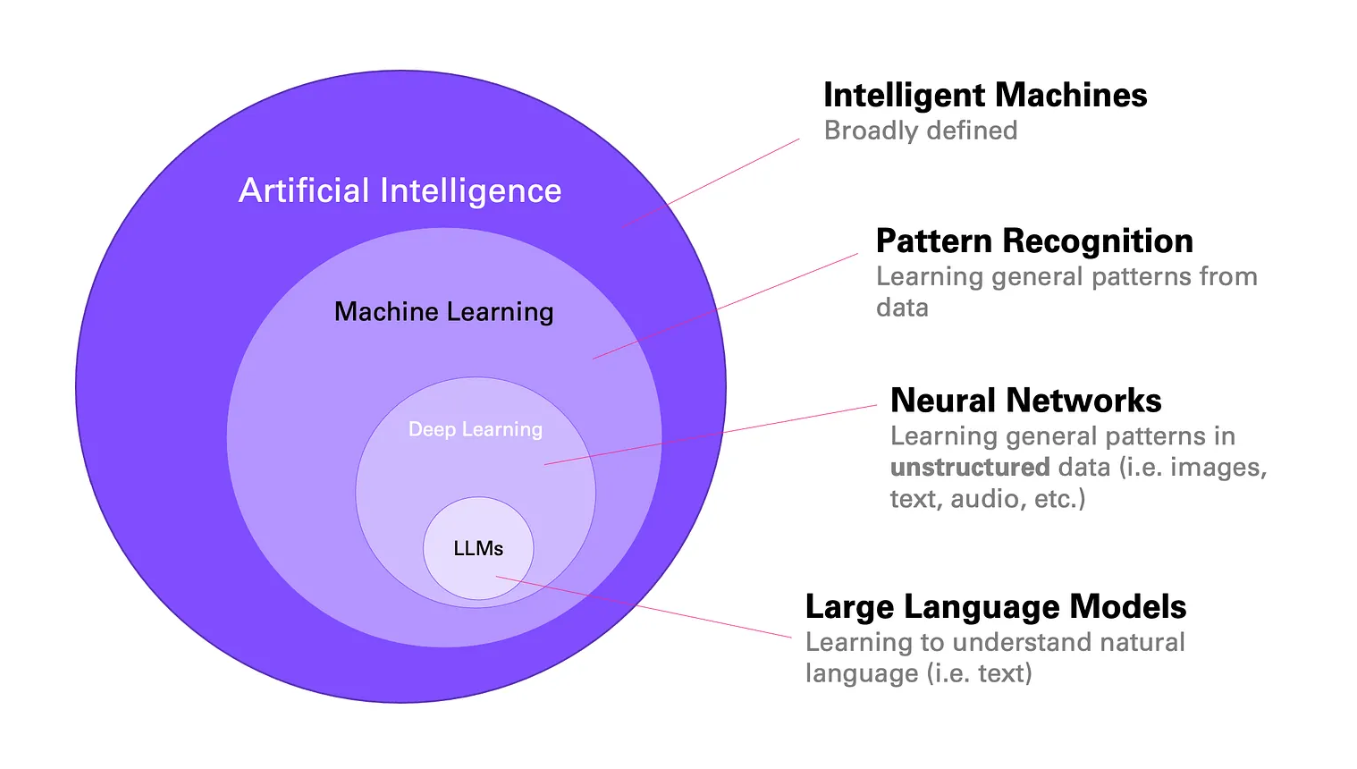
\includegraphics[width=0.5\textwidth]{LLMsphere.png}
  \caption{Artificiële intelligentie in lagen \autocite{Stoeffelbauer2023}}
  \label{fig:LLM-position}
\end{figure}

Large Language Modellen zijn geavanceerde AI-systemen die dienen om menselijke taal te verstaan, te genereren en te verwerken.
LLM's worden getraind op een grote hoeveelheid tekst wat vaak uit allerlei data zoals artikels of websites gehaald wordt. 
Volgens \textcite{Beelen2023} zorgen Deep Neural Networks ervoor dat LLM's natuurlijke taal verwerken op een gelijkaardige manier die vergelijkbaar is met de menselijke taalvaardigheid.
Deze hebben een grote vooruitgang gekend in 2017 door de paper van \textcite{VaswaniEtAl2017}. 
Hieruit kwam een nieuw mechanisme tot stand namelijk transformers wat bestaat uit Attentie blokken. 
Enkele voordelen die komen kijken bij het gebruiken van transformers zijn: 
\begin{itemize}
  \item Het kan lange sequenties verwerken.
  \item Het kan parallel sequenties verwerken.
  \item Het kan de relaties tussen de verschillende delen van de sequentie leren.
\end{itemize}
Hierdoor hebben transformer modellen een snellere trainingsperiode dan vorige neurale netwerken \autocite{aiml2023}.

\subsection{Transformers en de architectuur van LLM's}
\label{sec:architectuur-van-llms}
Omdat in dit onderzoek gebruik gemaakt wordt van LLM's is het nodig dat er dieper ingegaan wordt op de architectuur van deze modellen om een beter inzicht te krijgen hoe deze werken.
Een neuraal netwerk bestaat uit verschillende lagen. Enkele belangrijke blokken die gebruikt worden binnen de transformer laag zijn:
\begin{itemize}
  \item Self-Attention
  \item Cross-Attention
  \item Masked Self-Attention
\end{itemize}

Deze Attentie blokken worden gebruikt in de encoder en decoder van een transformer en stromen voort uit het onderzoek van \textcite{VaswaniEtAl2017}.

Transformers zijn een speciaal type van neurale netwerken die gebruik maken van verschillende Attentie blokken.
Attentie is een mechanisme dat gebruikt wordt om de relaties tussen verschillende delen van de invoersequenties te leren.
Een transformer bestaat uit een encoder en een decoder. 
Niet elke transformer bestaat uit zowel een encoder als een decoder het kan ook enkel encoder of decoder bevatten \autocite{Hoque2023}.
De encoder wordt gebruikt om de invoersequenties te verwerken en de decoder wordt gebruikt om de uitvoersequenties te genereren.
Zo is BERT van \textcite{DevlinEtAl2019} een transformer die enkel een encoder heeft en GPT van \textcite{RandfordEtAL2018} heeft enkel een decoder.
De transformer architectuur uit de paper van \textcite{VaswaniEtAl2017} kan gezien worden in figuur \ref{fig:transformer-model}. 

Self-Attention duidt dynamische gewichten toe aan verschillende elementen binnen de meegegeven sequentie, bijvoorbeeld bij woorden in een zin.
Dit laat het model toe om zich te concentreren op de meest relevante delen van de invoer, terwijl de invloed van minder cruciale delen wordt verminderd.
De invoersequentie wordt eerst in drie verschillende vectoren omgezet: Query, Key en Value.
De Query vector stelt een specifiek token uit de invoersequentie voor. De Key vector vertegenwoordigt alle tokens en de vector voor Value bevat de feitelijke inhoud die aan elk token is gekoppeld.
De similariteit tussen de Query en de Key vector wordt berekend aan de hand van het inwendig product van de twee vectoren.
Deze similariteit wordt gebruikt om de gewichten te berekenen die aan de Value vector worden toegekend \autocite{VaswaniEtAl2017}.

Masked Self-Attention is een variant van Self-Attention die gebruikt wordt in de decoder van een transformer.
In de decoder wordt er een mask gebruikt om enkel de vorige tokens te zien in de sequentie \autocite{VaswaniEtAl2017}.
Dit vermijdt dat er informatie van de toekomstige tokens gebruikt wordt. 
Zo kan de transformer niet "vals spelen"  tijdens het train proces.

Cross-Attention is een variant van Self-Attention die gebruikt wordt in de decoder van een transformer.
Deze laag gebruikt de informatie van de encoder en de vorige Attentie laag van de decoder om de uitvoersequenties te genereren.
De Query vector is de uitvoer van de vorige Attentie/Cross-Attention laag van de decoder en de Key en Value vector zijn de uitvoer van de encoder \autocite{VaswaniEtAl2017}.
Doordat de Cross-Attention laag informatie van zowel de encoder als decoder krijgt, kan het model de relaties tussen de verschillende delen van de invoersequenties leren.
Deze relaties worden dan gebruikt om de uitvoersequenties te genereren.

\begin{figure}[h]
  \centering
  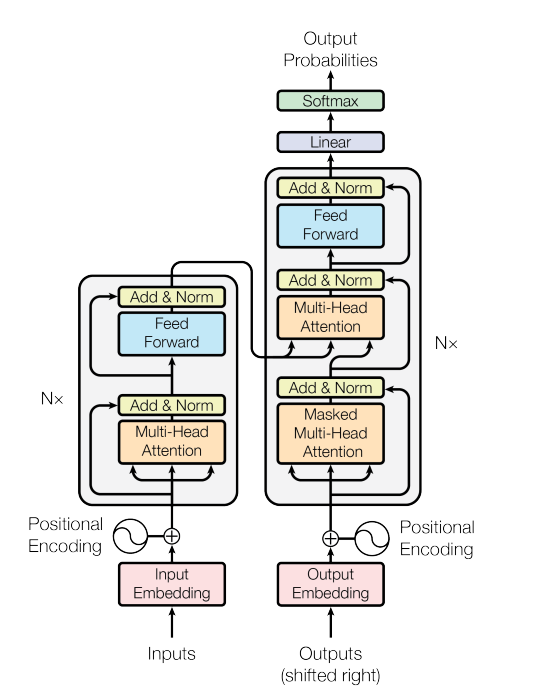
\includegraphics[width=0.5\textwidth]{transformer.png}
  \caption[Architectuur transformer model]{Transformer model architectuur \autocite{VaswaniEtAl2017}}
  \label{fig:transformer-model}
\end{figure}

\subsection{Trainen van LLM's}
\label{sec:trainen-van-llms}
Het trainen van LLM's is een complex proces dat veel tijd en rekenkracht vereist. Dit gebeurt in verschillende stappen.
De eerste fase begint bij het verzamelen van een grote hoeveelheid tekst die gebruikt wordt om het model te trainen.
Deze tekst wordt gehaald uit verschillende artikelen, websites, boeken en andere bronnen. 

Zo kan het volgende woord in een sequentie van tekst voorspeld worden.

Het model krijgt deze grote hoeveelheid tekst in de pre-training fase.
In deze fase leert de LLM grammatica, semantiek, taal patronen en factuele informatie \autocite{Cacic2023}.
Voordat de data meegegeven wordt aan het model moet de data gecleaned en geformatteerd worden.
Dit gebeurt in het tokenization proces. 
Hier wordt de tekst omgezet in tokens die het model kan verwerken \ref{fig:tokenization}.
Woorden kunnen kleiner gemaakt worden zodat de volledige tekst in het model past. 
Dit gebeurt wanneer het model een beperkte input capaciteit heeft \autocite{ElHousieny2023}.
Deze woorden worden dan omgezet wordt in embeddings en deze embeddings worden meegegeven aan het model om het te trainen.
Uit de data kunnen dan patronen gehaald worden met behulp van Transformers \ref{sec:architectuur-van-llms}, maar het is nog niet in staat om vragen of instructies te begrijpen.

\begin{figure}[h]
  \centering
  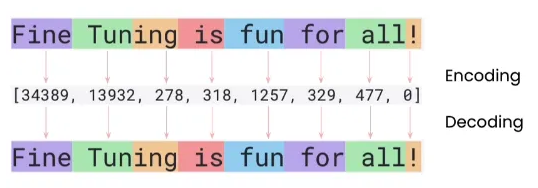
\includegraphics[width=0.5\textwidth]{tokenization.png}
  \caption[Tokenisatie van tekst]{Gesimplificeerde tokenisatie van tekst \autocite{TeeTracker2023}}
  \label{fig:tokenization}
\end{figure}

De volgende fase bestaat uit het trainen van het model op een dataset met instructies en het antwoord erop. 
Volgens \textcite{Das2024} is dit het gesuperviseerde Fine-Tunen van een LLM.
In deze fase probeert het model de patronen te leren die nodig zijn om vragen te beantwoorden of instructies te volgen.
Dit zorgt ervoor dat het model instructies kan volgen en vragen leert te beantwoorden.

Er kan gebruik gemaakt worden om het model specifiek aan de wensen van de mens te laten voldoen. Dit kan door het gebruiken van Reinfocement Learning met menselijke feedback \autocite{LambertEtAL2022}. 
Hierbij geeft de mens feedback aan het model en leert het model bij door deze feedback.

\subsection{Fine-Tuning van LLM's}
\label{sec:fine-tuning-van-llms}

Volgens \textcite{Peckham2024} kan het model achteraf nog extra getraind worden op een specifieke dataset zoals Python code of medische data.
Dit proces heet het Fine-Tunen van een LLM.
Een vereiste voor het Fine-Tunen van een LLM is dat de dataset een grote hoeveelheid data moet hebben.
Ook moet de dataset van hoge kwaliteit zijn en moet de dataset het onderwerp representatief voorstellen \autocite{Peckham2024}.

\subsection{Prompt Engineering}
\label{sec:prompt-engineering}

Prompt Engineering is een techniek die gebruikt wordt om de uitkomst van een LLM te beïnvloeden volgens \textcite{Google2023}.
Er wordt een prompt gegeven aan het model met duidelijke instructies over wat er verwacht wordt. 
Wanneer deze instructies niet voldoen, wordt de prompt iteratief aangepast en wordt de uitkomst geëvalueerd totdat de gewenste uitkomst is bereikt.
Dit iteratieve proces heet Prompt Engineering \autocite{Trad2024}.

Door het toevoegen van enkele voorbeelden aan de prompt kan het model beter begrijpen wat er verwacht wordt \autocite{OpenAi2024a}.
\begin{itemize}
  \item Geef structuur aan de prompt.
  \item Geef een rol mee.
  \item Geef een context.
  \item Geef een doel.
\end{itemize} 
Dit zijn de beste manieren om een prompt te structureren volgens \autocite{Google2023}.

\subsection{Bestaande LLM's}
\label{sec:bestaande-llms}

Momenteel zijn er verschillende LLM's die gebruikt worden voor verschillende taken.
Deze LLM's zijn getraind op verschillende datasets en hebben verschillende architecturen.
Het is belangrijk dat er een duidelijk beeld is van de verschillende LLM's en hun mogelijkheden. 
Met dit beeld kan er een goede keuze gemaakt worden voor het genereren van documentatie.

Eén van de grote spelers in de wereld van LLM's is OpenAI. OpenAI heeft verschillende LLM's ontwikkeld gaande van GPT \autocite{RandfordEtAL2018} tot GPT-4 \autocite{OpenAI2023}.
Het is getraind op een grote hoeveelheid data en heeft een grote capaciteit.
Een nadeel is dat GPT-4 een betalende service is \autocite{OpenAI2023}.

Een andere grote speler is Google. Google heeft verschillende LLM's ontwikkeld waaronder BERT van \textcite{DevlinEtAl2019} en Gemini \autocite{Google2024}.
BERT staat voor Bidirectional Encoder Representations from Transformers, een DL model waar elk output element verbonden is met elk input element \autocite{HashemiPour2024}.
BERT was een eerste stap in de wereld van LLM's voor Google. Sinds kort heeft \textcite{Google2024} een nieuwe LLM ontwikkeld genaamd Gemini.
Deze LLM is een sterke concurrent voor GPT-4 van \textcite{OpenAI2023}. 

Google \autocite{Google2024} bracht een model met verschillende versies uit: Gemini Pro, Gemini Ultra en Gemini Nano. 
Elke versie is gemaakt voor een specifiek doel. Zo is Gemini Nano het meest efficiënte model voor mobiele toestellen, terwijl Gemini Pro het beste model is voor het schalen van allerlei taken.
En Gemini Ultra is het meest capabele en grootste model van Google. Dit kan gebruikt worden voor complexe taken.
Een van de voordelen van Gemini is dat er een groot aantal input tokens meegegeven kunnen worden, namelijk 1 miljoen tokens \autocite{Google2024}.
Dit is aanzienlijk meer dan de 128 duizend tokens van GPT-4.

Een derde speler in de wereld van LLM's is Meta. Meta heeft verschillende LLM's ontwikkeld onder de naam LLama 2 \autocite{Meta2024}.
De LLama 2 familie bestaat uit verschillende LLM's die getraind zijn op verschillende data. Sommige zijn extra getraind voor specifiekere doeleinden.
Zo is er bijvoorbeeld een LLM getraind op Python code, genaamd Code LLama 2 van \textcite{Roziere2024}.
Een voordeel van de LLama 2 familie is dat deze LLM's open sourced zijn en dus voor iedereen toegankelijk zijn.

Antropic heeft ook een LLM ontwikkeld genaamd Claude \autocite{Anthropic2023}. 
Claude's capaciteiten zijn code generatie, het verstaan van meerdere talen, beelden analyseren en kan geavanceerde redeneringen geven.
Er bestaan 3 versies van Claude: Haiku, Sonnet en Opus.
Haiku is een lichte versie van Claude en Sonnet is de combinatie van performantie en snelheid. Opus is het intelligentste model dat complexe taken kan uitvoeren en begrijpen.
Claude is een betalende service en de prijzen zijn afhankelijk van de gekozen versie van Claude \autocite{Anthropic2023}.

De verschillen tussen deze LLM's zijn groot. Zo is er een verschil in capaciteit, trainingsdata en toegankelijkheid.
Het is belangrijk dat er een goede keuze gemaakt wordt voor het genereren van documentatie.
Deze keuze zal afhangen van de mogelijkheden van de LLM's en de doeleinden van de documentatie.

\begin{table}[h!]
\centering
\resizebox{\textwidth}{!}{
\begin{tabular}{|c|c|c|c|c|} 
  \hline
  Model & Input (1M tokens) & Output (1M tokens) & Context & Snelheid (t/s)\\ [0.5ex] 
  \hline
  GPT-4 Turbo \autocite{OpenAi2024} & \$10.00 & \$30.00 &  128k & 18\\ 
  \hline
  GPT-4 \autocite{OpenAi2024} & \$30.00 & \$60.00 &  128k & 21\\ 
  \hline
  GPT-3.5 Turbo \autocite{OpenAi2024} & \$0.50 & \$1.50 &  16k & 52\\
  \hline
  Gemini 1.5 Pro \textcite{Google2024} & \$3.50 & \$10.50 &  128k & 52\\
  \hline
  Code LLama \autocite{Meta2024} & \$0.90 & \$0.90 & 100k & 34\\
  \hline
  LLama 2 \autocite{Meta2024} & \$0.95 & \$1.00 & 100k & 34\\
  \hline
  Claude Opus \autocite{Anthropic2023} & \$15.00  & \$75 &  200k & 29\\
  \hline
  Claude Sonnet \autocite{Anthropic2023} & \$3.00  & \$15 &  200k & 61\\ 
  \hline
  Claude Haiku \autocite{Anthropic2023} & \$0.20  & \$1.20 &  200k & 102\\
  \hline
\end{tabular}}
\caption{Vergelijking van verschillende LLM's op basis van prijs (\$), context (aantal tokens) en snelheid (Tokens per seconde) \autocite{ArtificialAnalysis2024}}
\label{table:vgl-llms}
\end{table}

In de tabel \ref{table:vgl-llms} wordt er een vergelijking gemaakt tussen verschillende LLM's.
Hierin wordt er gekeken naar de prijs van de input en output tokens, de grootte van de context en het aantal tokens dat per seconde verwerkt kan worden.

\begin{table}[h!]
\centering
\resizebox{\textwidth}{!}{
\begin{tabular}{|c|c|c|c|}
\hline
Model & Coding & Beredenering en Kennis\\
\hline
GPT-4 Turbo \autocite{OpenAi2024} & 86\% & 85.4\% \\
\hline
GPT-4 \autocite{OpenAi2024} & 86\% & 88.4\% \\
\hline
GPT-3.5 Turbo \autocite{OpenAi2024} & 70\% & 73.2\% \\
\hline
Gemini 1.5 Pro \textcite{Google2024} & 82\% & 71.9\% \\
\hline
Code LLama \autocite{Meta2024} & /  & 67.8\% \\
\hline
LLama 2 \autocite{Meta2024} & 69\%  & / \\
\hline
Claude Opus \autocite{Anthropic2023} & 87\%  & / \\
\hline
Claude Sonnet \autocite{Anthropic2023} & 79\%  & / \\
\hline
Claude Haiku \autocite{Anthropic2023} & 75\%  & / \\
\hline
\end{tabular}}
\caption{Vergelijking LLM's op basis van beoordeling van menselijke evaluatie en MMLU \autocite{ArtificialAnalysis2024}}
\label{table:vgl-llms-eval}
\end{table}

In de tabel \ref{table:vgl-llms-eval} wordt een vergelijking gemaakt tussen verschillende LLM's tussen twee kolommen. 
De eerste kolom bevat de beoordeling van de coding mogelijkheden van het model gequoteerd met menselijke evaluatie. 
In de tweede kolom staat de quotering op basis van de MMLU een dataset opgesteld door \textcite{Hendrycks2020}.
MMLU staat voor het meten van de multitask taalbegrip capaciteiten van een model \autocite{Hendrycks2020}.
Beide kolommen staan uitgedrukt in procenten met 100\% als maximum.
Hieruit kan geconcludeerd worden dat GPT-4 en GPT-4 Turbo de beste scores behalen op beide vlakken.
Maar omdat er in dit onderzoek gezocht wordt naar een goedkope oplossing wordt er geconcludeerd uit beide tabellen dat GPT-3.5 Turbo de beste prijs/kwaliteit verhouding heeft.

%%=============================================================================
%% Methodologie
%%=============================================================================

\chapter{\IfLanguageName{dutch}{Methodologie}{Methodology}}%
\label{ch:methodologie}

%% TODO: In dit hoofstuk geef je een korte toelichting over hoe je te werk bent
%% gegaan. Verdeel je onderzoek in grote fasen, en licht in elke fase toe wat
%% de doelstelling was, welke deliverables daar uit gekomen zijn, en welke
%% onderzoeksmethoden je daarbij toegepast hebt. Verantwoord waarom je
%% op deze manier te werk gegaan bent.
%% 
%% Voorbeelden van zulke fasen zijn: literatuurstudie, opstellen van een
%% requirements-analyse, opstellen long-list (bij vergelijkende studie),
%% selectie van geschikte tools (bij vergelijkende studie, "short-list"),
%% opzetten testopstelling/PoC, uitvoeren testen en verzamelen
%% van resultaten, analyse van resultaten, ...
%%
%% !!!!! LET OP !!!!!
%%
%% Het is uitdrukkelijk NIET de bedoeling dat je het grootste deel van de corpus
%% van je bachelorproef in dit hoofstuk verwerkt! Dit hoofdstuk is eerder een
%% kort overzicht van je plan van aanpak.
%%
%% Maak voor elke fase (behalve het literatuuronderzoek) een NIEUW HOOFDSTUK aan
%% en geef het een gepaste titel.
\begin{figure}[h]
    \centering
    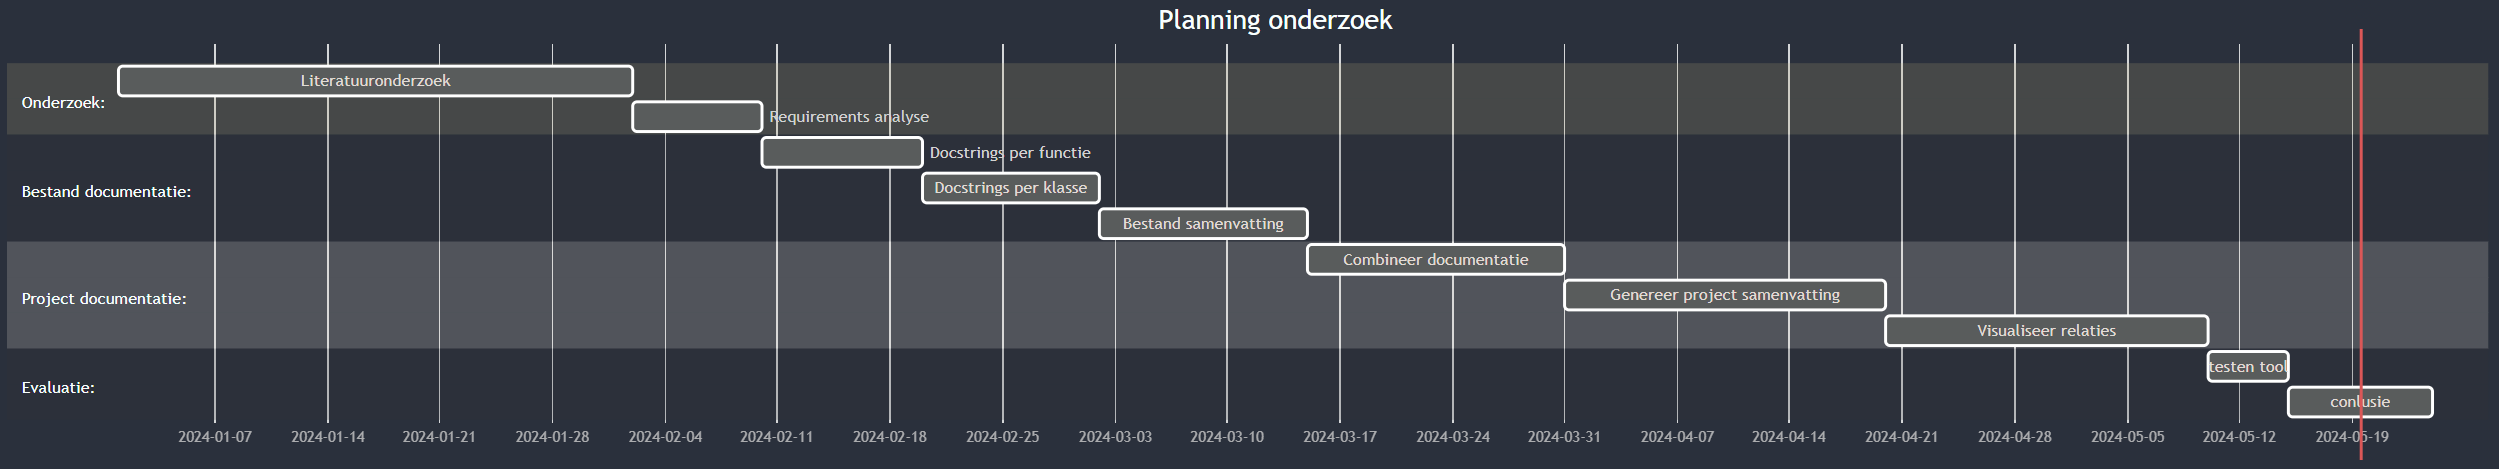
\includegraphics[width=1\textwidth]{flowchart.png}
    \caption{Tijdslijn onderzoek}
    \label{fig:flowchart}
\end{figure}

Het onderzoek is in drie fases opgedeeld. De eerste fase omvat de literatuurstudie.
In deze literatuurstudie wordt er onderzocht wat de huidige stand van zaken is omtent de technologie en mogelijkheden voor de documentatie van Python projecten met behulp van Large Language Modellen.
Zo wordt er gekeken naar wat LLM's zijn, hoe ze werken en wat bestaande tools zijn voor het genereren van documentatie.

Nadat er een duidelijk beeld gevormd is in de literatuurstudie, kan er begonnen worden aan de tweede fase.
Hier wordt er een tool ontwikkeld die een Python bestand kan analyseren en op basis daarvan documentatie kan genereren, aan de hand van het toevoegen van docstrings aan de code.
Dit doet het eerst per functie dan per klasse en uiteindelijk voor het gehele bestand. Dit kan later gebruikt worden om een samenvatting van het project te genereren in de volgende fase.
De uitkomst van deze fase is een tool die de documentatie van een Python bestand kan genereren. 
Door aan prompt engineering te doen, met het prompt dat meegegeven wordt aan de LLM, kunnen de bekomen docstrings accurater worden.
Verder wordt er gekeken naar hoe de documentatie van Python functies gebruikt kan worden voor het maken van een gehele samenvatting van het project.
Dit wordt gedaan op basis van huidige methoden om docstrings aan te maken en te gebruiken. 
Erna kunnen de verschillende docstrings met de bijhorende naam van de functie of klasse gebruikt worden om een samenvatting te genereren.
Deze informatie kan dan gegeven worden aan de Large Language Modellen om een samenvatting te genereren.

De derde fase beslaagt het documenteren van een geheel project.
Door de vorige fases te combineren, het documenteren van de individuele bestanden en het genereren van een samenvatting van het project, kan er een tool gemaakt worden die de documentatie van een geheel project kan genereren.
Deze documentatie bestaat uit de individuele documentatie van de bestanden en een samenvatting van het gehele project. 
Alsook wordt er gekeken naar hoe de relaties tussen de verschillende bestanden gevisualiseerd kunnen worden.

De laatste fase is het evalueren van de tool.
Hier wordt er gekeken naar de kwaliteit van de documentatie die de tool genereert.
Dit wordt gedaan door de documentatie van de tool te vergelijken met de handgeschreven documentatie van een project.
Dit wordt gedaan voor een bestand, een klein project en een groot project.

\section{Requirementsanalyse}
\label{sec:requirements-analyse}
De requirementsanalyse is een belangrijk onderdeel van het onderzoek. 
Hier wordt er gekeken naar wat de tool moet kunnen en wat de verwachtingen zijn van de tool.

\subsection{Functionele requirements}
\label{sec:functionele-requirements}
\subsubsection{Should Have:}
\begin{itemize}
    \item De tool moet in staat zijn om docstrings te genereren voor functies en klassen voor een Python bestand.\\
    De tool genereert docstrings voor functies en klassen in een Python bestand. Dit gebeurt door de code te analyseren en op basis daarvan een docstring te genereren.
    \item De tool moet in staat zijn om een samenvatting van een Python bestand te genereren.\\
    De tool maakt een samenvatting van een Python bestand. In deze samenvatting zitten de belangrijkste zaken van het bestand.
    Zijnde de functies en klassen die erin voorkomen en wat deze doen, alsook hun eventuele parameters en de uitkomst.
    \item De tool moet in staat zijn om een samenhangende samenvatting van een Python project te genereren.\\
    De tool dient een samenvatting te maken van een Python project. Deze samenvatting bestaat uit de individuele samenvattingen van de bestanden en een overkoepelende samenvatting van het project.
    Hierin staan alle functies en klassen die in het project voorkomen en wat deze doen, alsook hun eventuele parameters en de uitkomst.
    \item De tool moet in staat zijn om de relaties tussen de verschillende bestanden van een project te visualiseren.\\
    De tool visualiseert de relaties tussen de verschillende bestanden van een project. Zo is er geweten waar de bestanden naar verwijzen en van waar ze refereren.
\end{itemize}

\subsubsection{Could Have:}
\begin{itemize}
    \item De tool moet in staat zijn om de documentatie van een Python bestand te genereren in verschillende formaten.\\
    De tool genereert de documentatie van een Python bestand in verschillende formaten. Zo kan de gebruiker kiezen in welk formaat hij de documentatie wil.
    \item De tool moet in staat zijn om de relaties tussen de verschillende functies en klassen van een bestand te visualiseren op project niveau\\
    De tool visualiseert de relaties tussen de verschillende functies en klassen van een bestand op project niveau. Zo is er geweten waar de functies en klassen naar verwijzen en van waar ze refereren.
\end{itemize}

\subsubsection{Nice to Have:}
\begin{itemize}
    \item De tool moet in staat zijn om de documentatie van een Python bestand te genereren in verschillende talen.\\
    De tool genereert de documentatie van een Python bestand in verschillende talen. Zo kan de gebruiker kiezen in welke taal hij de documentatie wil.
    \item De tool moet in staat zijn om de documentatie van een Python bestand te genereren in verschillende stijlen.\\
    De tool genereert de documentatie van een Python bestand in verschillende stijlen. Zo kan de gebruiker kiezen in welke stijl hij de documentatie wil.
\end{itemize}

\subsection{Niet-functionele requirements}
\label{sec:niet-functionele-requirements}
\begin{itemize}
    \item De tool moet gebruiksvriendelijk zijn.\\
    De tool moet eenvoudig te gebruiken zijn. Dit betekent dat de tool intuïtief moet zijn en dat de gebruiker geen moeite moet doen om de tool te gebruiken.
    \item De tool moet betaalbaar zijn.\\
    Dit wil zeggen dat de tool geen hoge kosten met zich meebrengt.
    \item De tool moet snel werken.\\
    De tool moet snel werken. Dit betekent dat de tool snel de documentatie moet kunnen genereren. Sneller dan dat een persoon dit zou kunnen.
    \item De tool moet leesbare documentatie genereren.\\
    De documentatie die de tool genereert moet leesbaar zijn. Dit wil zeggen dat de documentatie duidelijk moet zijn en dat de gebruiker er gemakkelijk informatie uit kan halen.    
\end{itemize}

\section{Opstellen van een long-list tools}
\label{sec:long-list}
De long-list bestaat uit de verschillende tools die gebruikt kunnen worden voor het genereren van documentatie voor Pythonprojecten.
Deze tools worden onderzocht en vergeleken om te kijken welke het beste past bij de requirements van de tool.

De oplijsting van de tools is gebaseerd op de literatuurstudie en bestaat uit de volgende tools:
\begin{itemize}
\item Sphinx \autocite{Sphinx2023}\\
Een tool die gebruikt wordt voor het genereren van documentatie voor projecten met reeds een docstring. 
\item Doxygen \autocite{Doxygen2023}\\
Een tool die gebruikt wordt voor het genereren van documentatie voor projecten met reeds een docstring.
\item Pdoc \autocite{GallantHils2023}\\
Een tool die een API genereert voor Python projecten met reeds een docstring.
\item GPT4Docstrings \autocite{Trofficus2023}\\
Een tool die docstrings genereert voor Python projecten met behulp van GPT4 \textcite{OpenAI2023}.
\end{itemize}

Door de verschillende tools te onderzoeken en te vergelijken aan de hand van de requirementsanalyse kan er een keuze gemaakt worden welke tool het beste past bij de requirements van de tool.
Als er geen tool is die voldoet aan de requirements, kan er gekeken worden naar het combineren van verschillende tools of gebruiken van delen van verschillende tools om zo een eigen tool te maken.

Door eerst te kijken naar de programmeerttalen waarvoor de tools gebruikt kunnen worden, kan er al een eerste selectie gemaakt worden uit tabel \ref{table:vgl-tools}.
Zo kan er gekeken worden naar de tools die gebruikt kunnen worden voor Python projecten.
Vervolgens kan er gekeken worden naar het type documentatie dat de tools genereren.
Hierbij kan er gekeken worden naar de tools die docstrings genereren, aangezien dit de basis is voor het genereren van de gewenste documentatie.

\begin{table}[h!]
\centering
\resizebox{\textwidth}{!}{
\begin{tabular}{|c|c|c|c|c|}
\hline
Tool & docstrings & samenvatting bestand & samenvatting project & visualisatie \\ [0.5ex]
\hline
Doxygen & nee & ja & ja & ja \\
\hline
Sphinx & nee & ja & ja & nee \\
\hline
GPT4Docstrings & ja & nee & nee & nee \\
\hline
Pdoc & nee & ja & nee & nee \\
\hline
\end{tabular}}
\caption{Requirementsanalyse van de verschillende tools}
\label{table:ra-tools}
\end{table}

Uit deze tabel \ref{table:ra-tools} kan er geconcludeerd worden dat geen enkele tool voldoet aan de volledige requirements van de tool.
Doordat de Doxygen en Sphinx tools geen docstrings genereren en dit de basis is voor de documentatie, kunnen deze tools niet gebruikt worden.
Pdoc genereert enkel samenvattingen van een bestand dat reeds aangevuld is met docstrings en kan dus ook niet gebruikt worden.
Omdat GPT4Docstrings enkel docstrings genereert en geen samenvattingen van bestanden of projecten, kan er gekeken worden hoe deze tool dit doet.

% Voeg hier je eigen hoofdstukken toe die de ``corpus'' van je bachelorproef
% vormen. De structuur en titels hangen af van je eigen onderzoek. Je kan bv.
% elke fase in je onderzoek in een apart hoofdstuk bespreken.

%\input{...}
%\input{...}
%...

%%=============================================================================
%% Conclusie
%%=============================================================================

\chapter{Conclusie}%
\label{ch:conclusie}

% TODO: Trek een duidelijke conclusie, in de vorm van een antwoord op de
% onderzoeksvra(a)g(en). Wat was jouw bijdrage aan het onderzoeksdomein en
% hoe biedt dit meerwaarde aan het vakgebied/doelgroep? 
% Reflecteer kritisch over het resultaat. In Engelse teksten wordt deze sectie
% ``Discussion'' genoemd. Had je deze uitkomst verwacht? Zijn er zaken die nog
% niet duidelijk zijn?
% Heeft het onderzoek geleid tot nieuwe vragen die uitnodigen tot verder 
%onderzoek?

Het onderzoek had als doel de vraag te beantwoorden: "Hoe kan geautomatiseerde documentatiegeneratie met behulp van een Large Language Modellen (LLM) effectief worden toegepast op ongedocumenteerde Pythonprojecten om er duidelijke en overzichtelijke documentatie van te maken?"
Hiervoor werd er een tool ontwikkeld die voldeed aan de requirements die werden opgesteld in het onderzoek.
Enkele van deze requirements zijn dat de tool docstrings kan genereren dat er een bestand- en een projectsamenvatting gegenereerd kan worden en dat de tool zo goedkoop mogelijk moet zijn.
Voor deze vraag beantwoord kan worden is het belangrijk om te weten wat er juist bedoelt wordt met documentatie.
Onder documentatie wordt er begrepen dat er per bestand docstrings en een samenvatting van het bestand worden gegenereerd.
Voor een project wordt er een samenvatting van het project gegenereerd en een overzicht van alle bestanden in het project in de vorm van een graaf met de relaties.

Ook is het belangrijk om te weten wat enkele bestaande documentatietools zijn.
Tools zoals Sphinx, Doxygen en Pdoc zijn in staat om een gedocumenteerd project om te zetten in een website of API.
Deze tools zijn echter niet in staat om ongedocumenteerde projecten te documenteren.
Vervolgens werd de tool GPT4Docstrings besproken, deze tool is in staat om docstrings te genereren voor Pythonprojecten, de code van GPT4Docstrings werd gebruikt in de ontwikkeling van de tool.

Het documenteren van een bestand gebeurt door de code van het bestand in te lezen en per functie of klasse een docstring te genereren.
Vervolgens worden deze docstrings samengevoegd tot een bestandssamenvatting.
Voor een project te documenteren worden de verschillende bestanden in het project gedocumenteerd, worden de bestandssamenvatting samengevoegd tot een projectsamenvatting en wordt er een graaf gegenereerd met de relaties tussen de bestanden.

Er werd gekozen om een Large Language Model te gebruiken om de documentatie te genereren omdat deze modellen getraind zijn op grote hoeveelheden data en zowel code als natuurlijke taal kunnen begrijpen en genereren.
Door het gebruiken van GPT3.5-Turbo werd de tool zo goedkoop mogelijk gehouden.

Door de automatische gegenereerde documentatie van een project te evalueren met een vooropgesteld manueel gedocumenteerd project, werd er gekeken naar de verschillen en overeenkomsten tussen de documentatie van de tool en de handgeschreven documentatie.
De resultaten van de evaluatie tonen aan dat de documentatie van de tool en de handgeschreven documentatie gelijkaardig zijn.
Alhoewel er enkele fouten in de documentatie van de individuele bestanden zitten, blijft de gehele projectdocumentatie overzichtelijk en duidelijk.

Een verdere evaluatie van de tool kan gebeuren door een grote groep programmeurs verschillende projecten handmatig te laten documenteren en dit te chronometreren. 
Dezelfde projecten kunnen dan ook automatisch gedocumenteerd worden met de tool, de snelheid van de tool kan dan vergeleken worden met de snelheid van de programmeurs.
Daarna kan er een enquête afgenomen worden waarbij de programmeurs de keuze hebben tussen de handmatig gedocumenteerde projecten en de automatisch gedocumenteerde projecten.
Deze evaluatie kan dan gebruikt worden om de tool te verbeteren.



% % =============================

% Aangezien dit onderzoek een beperkte scope heeft, zijn er enkele uitbreidingen die kunnen worden toegevoegd om het onderzoek te verbeteren.
% Deze uitbreidingen kunnen helpen om de resultaten van het onderzoek te verbeteren en om de tool verder te ontwikkelen.

% Zo kan er gekeken worden naar het genereren van documentatie voor andere programmeertalen.
% Deze bachelorproef focust zich op Python, maar het is mogelijk om de tool uit te breiden naar andere programmeertalen.
% Aangezien een Large Language Model zoals GPT \autocite{OpenAi2024} ook getraind zijn op andere programmeertalen.

% Ook kan er gekeken worden naar hoe projecten met syntax fouten of andere problemen gedocumenteerd kunnen worden.
% Dit is belangrijk omdat de tool nu enkel werkt op projecten die correcte syntax hebben.
% Deze fouten kunnen eruit gehaald worden door de code eerst door een linter te halen en dan pas de documentatie te genereren.
% De bekomen syntax fouten kunnen dan meegegeven worden aan een model om zo een bestand te genereren zonder syntax fouten.

% Een andere uitbreiding is kijken naar hoe de documentatie geëvalueerd kan worden.
% Omdat dit nu slechts manueel gebeurt, op basis van gezond verstand. 
% Er kan gekozen worden om enquêtes af te nemen bij programmeurs om zo de documentatie te evalueren.
% De evaluatie van de respondenten gaat echter slechts relatief zijn, omdat de respondenten beoordelen op basis van kennis van de programmeertaal. 
% Of er kan gekeken worden naar hoe de documentatie van de tool vergeleken kan worden met de documentatie van de programmeur zelf.
% Hier is het belangrijk om te kijken naar de verschillen en overeenkomsten tussen de documentatie van de tool en de documentatie van de programmeur.

% Een laatste voorbeeld van een uitbreiding is om te kijken naar hoe verschillende Large Language Models presteren op het genereren van documentatie.
% Zo kan er gekozen worden tussen modellen zoals GPT-4 \autocite{OpenAI2023}, LLama 2 \autocite{Meta2024}, Gemini \autocite{Google2024}, \dots

% Sommige modellen hebben een groter context window dan andere modellen, zo zou er meer informatie meegegeven kunnen worden aan het model.
% En het zou mogelijk een beter resultaat kunnen geven.

%---------- Bijlagen -----------------------------------------------------------

\appendix

\chapter{Onderzoeksvoorstel}

Het onderwerp van deze bachelorproef is gebaseerd op een onderzoeksvoorstel dat vooraf werd beoordeeld door de promotor. Dat voorstel is opgenomen in deze bijlage.

%% TODO: 
%\section*{Samenvatting}

% Kopieer en plak hier de samenvatting (abstract) van je onderzoeksvoorstel.
\begin{abstract}
    Documentatie van een Python project is belangrijk, maar het is een tijdrovende taak en het wordt vaak niet grondig gedaan.
    Deze bachelorproef aan de HoGent onderzoekt het automatisch genereren van documentatie voor python projecten met behulp van Large Language Modellen.
    Er wordt een tool ontwikkeld die de Python code en de relaties tussen de verschillende bestanden analyseert en op basis daarvan een overzichtelijke documentatie genereerd.
    Er wordt gekeken naar hoe de documentatie van Python functies gebruikt kunnen worden voor het maken van een gehele samenvatting van het project.
    Dit wordt gedaan op basis van huidige methoden om docstrings aan te maken en te gebruiken.
    Deze informatie kan dan gegeven worden aan de Large Language Modellen om een samenvatting te genereren.
    
    Er worden verschillende Python projecten verzameld en geanalyseerd om te kijken hoe de documentatie gegenereerd kan worden.
    Dan worden er LLMs getraind op basis van deze projecten en wordt er gekeken naar hoe de documentatie gegenereerd kan worden.
    De gegenereerde documentatie kan dan vergeleken worden met de huidige documentatie van de projecten om dit te evalueren.
    Ook zal er gevraagd worden aan enkele programmeurs om de documentatie te evalueren.
    
    Op basis van deze feedback kan het model gefinetuned worden. Er kan gekeken worden naar de mogelijke verbeteringspunten zodat er uiteindelijk een betere documentatie van het project ontstaat.
    Het resultaat is dat er een tool is die de documentatie van een Python project kan genereren.
    Dit resultaat maakt het mogelijk om de gegenereerde samenvatting van een Python project te lezen. 
    De lezer kan dan stukken gebruiken uit het project of er verder mee aan de slag gaan.
\end{abstract}

% Verwijzing naar het bestand met de inhoud van het onderzoeksvoorstel
%---------- Inleiding ---------------------------------------------------------

\section{Introductie}%
\label{sec:introductie}

Documentatie is belangrijk wanneer er aanpassingen moeten gebeuren aan de code van een project. Ook moet een iemand anders de code kunnen begrijpen voordat de code gebruikt kan worden binnen een ander project.
Hoe kan geautomatiseerde documentatiegeneratie met behulp van Large Language Modellen (LLM) effectief worden toegepast om een duidelijk overzichten en informatieve beschrijvingen te produceren voor Python projecten?

Het is belangrijk dat de skill of de knowhow van een project gedeeld kan worden met anderen. 
Door het toepassen van documentatie kan deze kennis makkelijk vergaard worden door andere geïnteresseerden.
Het is dus een belangrijk dat er aan documentatie gedaan wordt en dat deze up-to-date blijft. 

Documentatie is iets dat veel tijd kost, dat vaak niet gemaakt wordt en het is iets dat up-to-date gehouden moet worden.
Het gebruiken ervan kan ervoor zorgen dat er geen dubbel werk gedaan moet worden. Een tool die dit proces kan versnellen / automatiseren zou een grote meerwaarde zijn.
De tool bestaat uit een geautomatiseerde documentatie LLM die de project code analyseert en samenvat in een document. 
Dit geeft de werknemers de moegelijkheid om zich in te lezen in het project en erna zelf aanpassingen te maken of stukken code te gebruiken voor een ander project.

Het eindresultaat van deze bachelorproef is een Proof of Concept (PoC) van een geautomatiseerde tool die de project code analyseert en er documentatie van genereert.
De gegenereerde documentatie laat het toe om het project te begrijpen zonder er te veel tijd aan te besteden.

%---------- Stand van zaken ---------------------------------------------------

\section{Literatuurstudie}%
\label{sec:Literatuurstudie}

Wat is documentatie binnen Python projecten en wat zijn de huidige tools?
Voor de taal Python bestaan er al verschillende tools die documentatie genereren voor blokken code zoals pdoc \autocite{GallantHils2023} en Sphinx \autocite{Sphinx2023}. 
Met behulp van de sphinx autodoc functie \autocite{Sphinx2023} kan een python functie omschreven worden in een docstring.
Een docstring is een blok tekst dat de werking van een python functie omschrijft. Door deze beknopte blok tekst wordt er duidelijk wat de functie doet.
Deze docstrings kunnen mogelijks gebruikt worden bij het maken van een document dat het project omschrijft.

Er is ook al onderzoek gedaan naar het automatisch genereren van documentatie van code blokken met behulp van een Neural Attention Model (NAM) \autocite{IyerEtAl2016}.
Dit onderzoek heeft gekeken naar het genereren van hoogstaande samenvattingen van source code. 
Het maakt gebruik van neurale netwerken die stukken C\# code en SQL queries omzetten naar zinnen die de code omschrijven. 
Dit helpt bij het begrijpen van stukken code maar niet van een geheel project waar meerdere bestanden bij betrokken zijn.

Hoe kunnen Large Language Modellen gebruikt worden om documentatie te genereren?
Large Language Modellen zijn neurale netwerken die getraind worden op grote hoeveelheden tekst. 
Deze modellen kunnen tekst genereren op basis van een gegeven input. De mogelijkse invoer in deze bachelorproef kan dan een python project zijn, of de docstrings van verschillende functies in een project.
Er wordt dan verwacht dat het een samenvatting maakt van het project of van de functies.

Ook kan er gekeken worden naar GitHub README.md bestanden. Dit zijn bestanden waarin de werking van een project kort wordt uitgelegd. Deze zijn echter niet altijd makkelijk te lezen. 
Volgens de studie \textcite{GaoEtAl2023} kan de tekst vereenvoudigd worden terwijl steeds de correcte betekenis te behouden, en dit aan de hand van een transfer learning model.
Het gebruik van LLMs en het automatisch code documentatie met behulp van syntax bomen wordt onderzocht in \textcite{Procko2023} voor de C\# en .NET programeertalen.
In deze studie wordt er gekeken naar het gebruik van LLMs specifiek GPT-3.5 en GPT-4 om code te documenteren.

In de studie van \textcite{McBurneyMcMillan2014} wordt onderzocht hoe er automatisch documentatie gegenereerd kan worden voor Java code, specifiek naar hoe de methodes met elkaar verbonden zijn en welke rol ze spelen binnen het project.
Dit is een mooi voorbeeld van wat ik wil bereiken met deze bachelorproef, een samenhangend geheel van verschillende bestanden van een python project die samen een duidelijk overzicht geven van de werking van het project.
Hoe kunnen LLMs gebruikt worden om automatisch documentatie te genereren voor python projecten.
De gegenereerde samenvatting van het gehele project geeft de lezer ervan de mogelijkheid het project te gebruiken of aan te passen zonde de totale project code te ontleden.

%---------- Methodologie ------------------------------------------------------
\section{Methodologie}%
\label{sec:methodologie}

Hier beschrijf je hoe je van plan bent het onderzoek te voeren. Welke onderzoekstechniek ga je toepassen om elk van je onderzoeksvragen te beantwoorden? 
Gebruik je hiervoor literatuurstudie, interviews met belanghebbenden (bv.~voor requirements-analyse), experimenten, simulaties, vergelijkende studie, risico-analyse, PoC, \ldots?

Valt je onderwerp onder één van de typische soorten bachelorproeven die besproken zijn in de lessen Research Methods (bv.\ vergelijkende studie of risico-analyse)? 
Zorg er dan ook voor dat we duidelijk de verschillende stappen terug vinden die we verwachten in dit soort onderzoek!

Vermijd onderzoekstechnieken die geen objectieve, meetbare resultaten kunnen opleveren. 
Enquêtes, bijvoorbeeld, zijn voor een bachelorproef informatica meestal \textbf{niet geschikt}. 
De antwoorden zijn eerder meningen dan feiten en in de praktijk blijkt het ook bijzonder moeilijk om voldoende respondenten te vinden. 
Studenten die een enquête willen voeren, hebben meestal ook geen goede definitie van de populatie, 
waardoor ook niet kan aangetoond worden dat eventuele resultaten representatief zijn.

Uit dit onderdeel moet duidelijk naar voor komen dat je bachelorproef ook technisch voldoen\-de diepgang zal bevatten. 
Het zou niet kloppen als een bachelorproef informatica ook door bv.\ een student marketing zou kunnen uitgevoerd worden.

Je beschrijft ook al welke tools (hardware, software, diensten, \ldots) je denkt hiervoor te gebruiken of te ontwikkelen.

Probeer ook een tijdschatting te maken. Hoe lang zal je met elke fase van je onderzoek bezig zijn en wat zijn de concrete \emph{deliverables} in elke fase?

%---------- Verwachte resultaten ----------------------------------------------
\section{Verwacht resultaat, conclusie}%
\label{sec:verwachte_resultaten}

Hier beschrijf je welke resultaten je verwacht. Als je metingen en simulaties uitvoert, kan je hier al mock-ups maken van de grafieken samen met de verwachte conclusies. 
Benoem zeker al je assen en de onderdelen van de grafiek die je gaat gebruiken. 
Dit zorgt ervoor dat je concreet weet welk soort data je moet verzamelen en hoe je die moet meten.

Wat heeft de doelgroep van je onderzoek aan het resultaat? Op welke manier zorgt jouw bachelorproef voor een meerwaarde?

Hier beschrijf je wat je verwacht uit je onderzoek, met de motivatie waarom. Het is \textbf{niet} erg indien uit je onderzoek andere 
resultaten en conclusies vloeien dan dat je hier beschrijft: het is dan juist interessant om te 
onderzoeken waarom jouw hypothesen niet overeenkomen met de resultaten.



%%---------- Andere bijlagen --------------------------------------------------
% TODO: Voeg hier eventuele andere bijlagen toe. Bv. als je deze BP voor de
% tweede keer indient, een overzicht van de verbeteringen t.o.v. het origineel.
%\input{...}

%%---------- Backmatter, referentielijst ---------------------------------------

\backmatter{}

\setlength\bibitemsep{2pt} %% Add Some space between the bibliograpy entries
\printbibliography[heading=bibintoc]

\end{document}
